%%
%% 2019 07 04 Ph. G. Freimann
%%
\section{Strahlensätze}\index{Strahlensätze}
\sectuntertitel{Frau zum Arzt: Das Röntgenbild von meinem Mann können Sie sich sparen: Ich durchschaue ihn auch so.}

%%%%%%%%%%%%%%%%%%%%%%%%%%%%%%%%%%%%%%%%%%%%%%%%%%%%%%%%%%%%%%%%%%%%%%%%%%%%%%%%%
\theorieTALSGeom{56}{1.4}

\subsection*{Lernziele}
\begin{itemize}
  \item Anwenden der Strahlensätze
\end{itemize}

\raisebox{2cm}{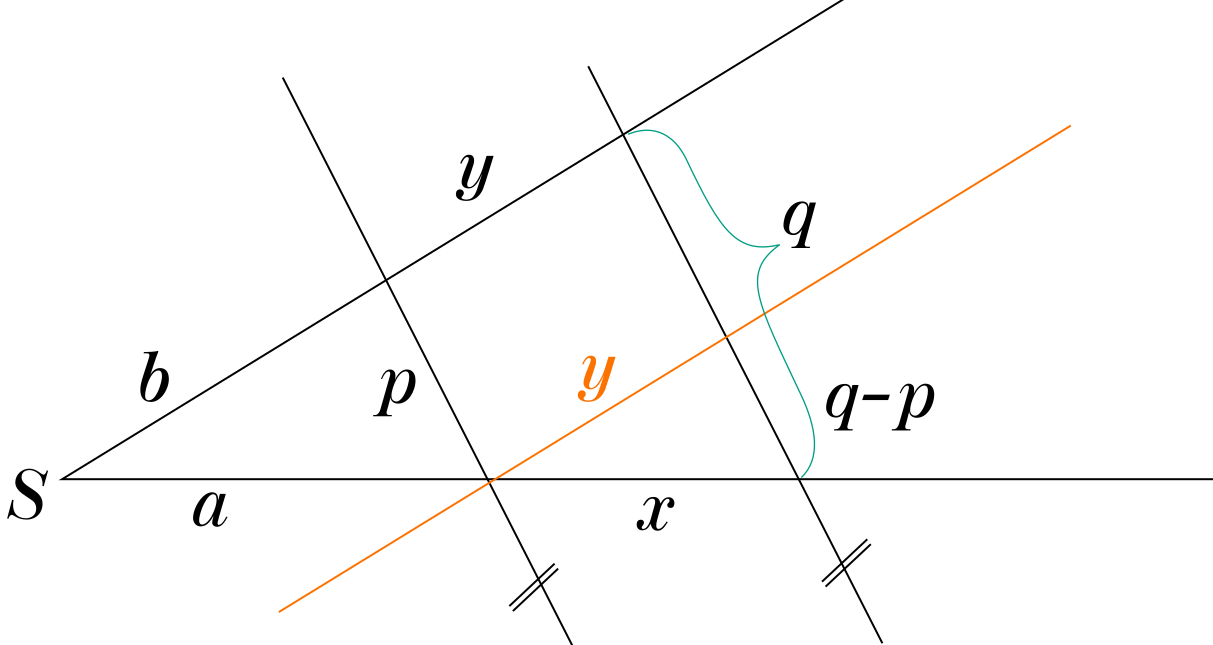
\includegraphics[width=8cm]{tals/plani/img/strahlensatz.png}}\\

Die drei folgenden Dreiecke sind ähnlich (Symbol $\sim{}$)
$$\Delta ( a, p, b)  \sim{} \Delta (a+x, q, b+y)  \sim{} \Delta (x, q-p, y)$$
Somit gelten \zB{} folgende Ähnlichkeiten...
$$a : (a+x) = p : q = b : (b+y)$$
...aber auch:
$$a:x = b:y$$

\subsection*{Aufgaben}
\TALSGeomAadB{57 \zB}{225. a) b) 226. 231.}
\GESOAadB{???}{???}

